\documentclass[11pt,a4paper]{article}
\usepackage[T2A]{fontenc}
\usepackage[utf8]{inputenc}
\usepackage[russian]{babel}
\usepackage[a4paper,margin=2.2cm]{geometry}
\usepackage{amsmath,amssymb,amsthm,mathtools}
\usepackage{graphicx}
\usepackage{booktabs,array,longtable}
\usepackage{tikz}
\usetikzlibrary{arrows.meta,decorations.pathmorphing,patterns}
\usepackage[hidelinks]{hyperref}
\usepackage{xcolor}

\newtheorem{proposition}{Утверждение}
\theoremstyle{definition}
\newtheorem{definition}{Определение}
\theoremstyle{remark}
\newtheorem{remark}{Замечание}

\newcommand{\jump}[1]{[\![#1]\!]}
\newcommand{\avg}[1]{\langle #1\rangle}
\newcommand{\bw}{\mathbf w}
\newcommand{\bF}{\mathbf F}
\newcommand{\bv}{\mathbf v}
\newcommand{\bT}{\mathbf T}
\newcommand{\br}{\mathbf r}
\newcommand{\lean}[1]{\texttt{\detokenize{#1}}}
\definecolor{fastc}{HTML}{111111}
\setlength{\emergencystretch}{3em}
\sloppy
\definecolor{slowc}{HTML}{0A8F2A}

\title{Математическая модель взаимодействия волн\\ при серии ударов по границе\\ предварительно деформированной разномодульной упругой среды}
\author{Проект \texttt{deformations-2d} (по мотивам диссертации О.\,В.~Дудко, 1998)}
\date{}

\begin{document}
\maketitle

\begin{abstract}
Описана математическая модель, по которой веб-приложение \texttt{deformations-2d} (вкладка
<<Серия ударов>>, метод <<ударные волны + сетка>>) рассчитывает одномерные нестационарные
волновые процессы в разномодульной изотропной упругой среде Мясникова--Олейникова при
кусочно-постоянном законе движения границы. Решение строится как композиция точно решаемых
<<элементарных взаимодействий>>: изменение скорости границы, отражение волны от границы, встреча
двух разрывов, непрерывное взаимодействие ударной волны с гладкой волной. Для каждого из них
выписаны уравнения, число неизвестных и условия, по которым выбирается тип рождающихся волн.
Гладкие области (вееры) рассчитываются методом конечных объёмов второго порядка между выделенными
разрывами. Подробно разобран вариант <<материал 2, слабое предсжатие, удар\,--\,рывок\,--\,удар>>:
перечислены все возникающие встречи и их исход. Алгебраические соотношения модели (26 утверждений)
формально проверены в системе Lean~4 с библиотекой Mathlib. Аналитические утверждения, которые
формализации не поддаются, проверены численно. При выводе формул найдена и исправлена ошибка
знака в граничном условии программы.
\end{abstract}

\tableofcontents

%======================================================================
\section{Постановка задачи}

\subsection{Среда}
Рассматривается изотропная упругая среда с упругим потенциалом Мясникова--Олейникова
(формула (1.9) диссертации):
\begin{equation}\label{eq:W}
W = \tfrac12\lambda J_1^2 + \mu J_2 - \nu J_1\sqrt{J_2} + \alpha\frac{J_1^3}{\sqrt{J_2}} + \beta\frac{J_3}{\sqrt{J_2}},
\qquad J_k = \operatorname{tr}\,(\varepsilon^k),
\end{equation}
где $\varepsilon$ --- тензор малых деформаций, $\lambda,\mu$ --- модули Ламе, $\nu,\alpha,\beta$
--- модули разномодульности. Потенциал однороден второй степени, но не аналитичен в нуле:
отклик на растяжение и сжатие различен. Напряжения (формула (1.10)):
\begin{equation}\label{eq:sigma}
\sigma = A\,\delta + B\,\varepsilon + C\,\varepsilon^2,\quad
A=\lambda J_1-\nu\sqrt{J_2}+3\alpha\varphi J_1,\quad
B=2\mu-\nu\varphi-\alpha\varphi^3-\beta\eta,\quad
C=\frac{3\beta}{\sqrt{J_2}},
\end{equation}
$\varphi = J_1/\sqrt{J_2}$, $\eta = J_3/J_2^{3/2}$.

Все модули далее отнесены к $\lambda+2\mu$, скорости --- к $c_1=\sqrt{(\lambda+2\mu)/\rho}$,
координата --- к длине $L$ показанного участка, время --- к $L/c_1$.
Для материала~2 (стр.~109 диссертации) $\lambda=0{,}33803$, $\mu=0{,}33099$, $\nu=0{,}14789$,
$\alpha=0{,}08451$, $\beta=-0{,}02113$.

\subsection{Одномерная деформация}
Перемещения зависят только от $x=x_1$ и $t$: $\mathbf u = \mathbf u(x,t)$. Градиент перемещений
задаётся вектором $(p,g,s) = (u_{1,1}, u_{2,1}, u_{3,1})$, отличные от нуля компоненты тензора
деформаций --- $\varepsilon_{11}=p$, $\varepsilon_{12}=g/2$, $\varepsilon_{13}=s/2$. Тогда
\begin{equation}\label{eq:J}
J_1 = p,\qquad J_2 = p^2+\tfrac12(g^2+s^2),\qquad J_3 = p^3 + \tfrac34\,p\,(g^2+s^2),
\end{equation}
а вектор напряжений на площадке $x=\mathrm{const}$ равен
\begin{equation}\label{eq:T}
\bT = (\sigma_{11},\sigma_{21},\sigma_{31}) = \Bigl(A + Bp + C\bigl(p^2+\tfrac{g^2+s^2}{4}\bigr),\; k g,\; k s\Bigr),\qquad k=\frac{B+Cp}{2}.
\end{equation}
Формулы \eqref{eq:J}, \eqref{eq:T} --- следствие \eqref{eq:sigma} (теоремы \lean{J1_eq}, \lean{J2_eq},
\lean{J3_eq}, \lean{traction_eq}, приложение~\ref{app:lean}). Кроме того, $\bT = \partial W/\partial(p,g,s)$:
это проверено численно (тест <<$T=\partial W/\partial F$>>, раздел~\ref{sec:verify}).

Касательное напряжение коллинеарно сдвигу: $(\sigma_{21},\sigma_{31}) = k\,(g,s)$. Поэтому при
нормальном ударе по среде с предварительным сдвигом в плоскости $x_1x_3$ ($g_0=0$) компонента $g$
остаётся нулевой, и состояние описывается вектором
\[
\bw = (p,\,s,\,v_1,\,v_3),\qquad \bF=(p,s),\quad \bv=(v_1,v_3),\quad \bT(\bF)=(\sigma_{11},\sigma_{31}).
\]

\subsection{Система законов сохранения}
В лагранжевой координате уравнения движения и условия совместности $\bF_t = \bv_x$,
$\bv_t = \bT(\bF)_x$ записываются в дивергентной форме
\begin{equation}\label{eq:cons}
\bw_t + \mathbf f(\bw)_x = 0,\qquad \mathbf f(\bw) = -\bigl(v_1,\;v_3,\;T_1(\bF),\;T_3(\bF)\bigr).
\end{equation}
Начальное состояние --- однородная предварительная деформация в покое:
$\bw(x,0) = (p_0, s_0, 0, 0)$. На границе $x=0$ задана скорость:
\begin{equation}\label{eq:bc}
\bv(0,t) = (d(t),\,0),\qquad d(t) = \sum_k d_k\,\mathbf 1\{t_k\le t<t_k+\Delta t_k\},
\end{equation}
$d>0$ --- граница вдавливается (удар, сжатие), $d<0$ --- рывок наружу (растяжение).
Справа --- свободный выход волн ($x=X$ выбирается так, чтобы к концу расчёта все волны
оставались на участке; выходящие потоки учитываются в балансах).

\begin{table}[h]
\centering
\caption{Разбираемый вариант (снимок экрана приложения).}\label{tab:case}
\begin{tabular}{@{}l p{0.62\textwidth}@{}}
\toprule
Материал & 2 (нормированные модули выше)\\
Предварительная деформация & $p_0=-0{,}0005$ (слабое сжатие), $s_0=0{,}001$\\
Воздействия & $d=0{,}002$ на $[0;\,0{,}25)$, $d=-0{,}002$ на $[0{,}25;\,0{,}5)$, $d=0{,}002$ на $[0{,}5;\,0{,}75)$\\
Метод & ударные волны выделены, вееры на сетке (400 ячеек на $L$, огрублено до 2400 ячеек)\\
Расчёт & <<до затухания>>: $t\le 10{,}11$, $x\le 11{,}24$\\
\bottomrule
\end{tabular}
\end{table}

%======================================================================
\section{Волны и условия на разрывах}

\subsection{Характеристики}
Якобиан потока $J = \partial\mathbf f/\partial\bw$ действует как
$J(\mathbf e_F,\mathbf e_v) = -(\mathbf e_v,\;A\mathbf e_F)$, где
\begin{equation}
A(\bF) = \frac{\partial\bT}{\partial\bF} = \begin{pmatrix} a & b\\ b & d\end{pmatrix}
\end{equation}
--- акустическая матрица. Она симметрична, потому что $\bT$ --- градиент потенциала.
Собственные значения
\begin{equation}\label{eq:eig}
\lambda_\pm = \frac{a+d}{2}\pm D,\qquad D=\sqrt{\Bigl(\frac{a-d}{2}\Bigr)^2+b^2},
\end{equation}
собственные векторы $\br_\pm \parallel (b,\;\lambda_\pm-a)$ ортогональны (\lean{eigen_char},
\lean{eigen_vec}, \lean{eigen_orth}). Если $A$ положительно определена, то $0<\lambda_-\le\lambda_+$
(\lean{eigen_pos}): система \eqref{eq:cons} гиперболична, а четыре характеристические скорости равны
\[
-c_f < -c_s < c_s < c_f,\qquad c_f=\sqrt{\lambda_+}\ \text{(квазипродольная)},\quad c_s=\sqrt{\lambda_-}\ \text{(квазипоперечная)}.
\]
Семейства нумеруются $m=0,1,2,3$ в этом порядке. Положительная определённость $A$ в
рассматриваемых состояниях проверена численно.

Главная особенность разномодульной среды видна на рис.~\ref{fig:speeds}. Когда $p$ проходит
через ноль (точнее, интервал $|p|\lesssim s$), $c_f$ меняется на $\approx17\,\%$: от $1{,}080$ в
сжатой зоне ($p\approx-0{,}0024$) до $0{,}922$ в растянутой ($p\approx0{,}0016$). Скорость $c_s$
меняется от $0{,}667$ до $0{,}510$. Зависимость $c_f(p)$ немонотонна вблизи $p=0$, то есть
семейство не является истинно нелинейным во всей области.

\begin{figure}[h]
\centering
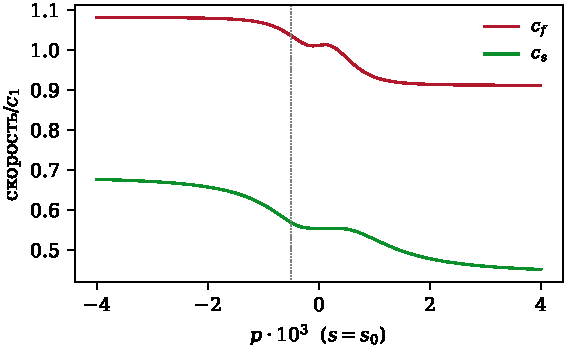
\includegraphics[width=0.62\textwidth]{figures/speeds.pdf}
\caption{Скорости характеристик материала~2 при $s=s_0$; пунктир --- $p_0$.}\label{fig:speeds}
\end{figure}

\subsection{Простые волны}
Гладкое решение вида $\bw(\xi)$, $\xi = x/(t-t_*)$ (центрированный веер) существует, только если
$\xi = \sigma_m(\bw)$ и $\bw'(\xi)\parallel\mathbf e_m$. Здесь
\begin{equation}\label{eq:simple}
\mathbf e_m = (\br_m,\; -\sigma_m\br_m),\qquad J\,\mathbf e_m = \sigma_m\mathbf e_m
\end{equation}
(\lean{simple_wave_dir}). Вдоль веера $\sigma_m$ должна возрастать от тыла к фронту: веер
расходится. Ширина веера в момент $\tau$ после рождения равна $(\sigma_m^{\text{фронт}}-\sigma_m^{\text{тыл}})\,\tau$.

\subsection{Разрывы}
На разрыве, движущемся со скоростью $G$, выполняется $\jump{\mathbf f} = G\jump{\bw}$ ($\jump{\cdot}$ ---
значение справа минус значение слева). Для \eqref{eq:cons} это равносильно условиям (2.40)--(2.42)
диссертации:
\begin{equation}\label{eq:rh}
\jump{\bv} = -G\jump{\bF},\qquad \jump{\bT} = G^2\jump{\bF}
\end{equation}
(\lean{rh_iff}). Отсюда скачки $\jump{\bT}$ и $\jump{\bF}$ коллинеарны, и
\begin{equation}\label{eq:G2}
G^2 = \frac{\jump{\bT}\cdot\jump{\bF}}{|\jump{\bF}|^2}
\end{equation}
(\lean{shock_speed}). Для линейного материала скорость разрыва характеристическая
(\lean{linear_shock_is_characteristic}).

Ударная адиабата семейства $m$ из состояния $\bF_a$ строится так:
$\bF_b = \bF_a + \varepsilon(\br_m + \eta\,\mathbf t)$, $\mathbf t\perp\br_m$, где $\eta(\varepsilon)$
находится из коллинеарности $\jump{\bT}\times\jump{\bF}=0$, а $G^2$ --- из \eqref{eq:G2}. Вектор $\br_m$
ориентирован в сторону роста $\lambda_m$, поэтому $\varepsilon>0$ соответствует сжимающему скачку,
а $\varepsilon<0$ --- разрежению.

\subsection{Энергия и допустимость}
Плотность энергии $E = W(\bF) + \tfrac12|\bv|^2$ удовлетворяет в гладких областях закону
сохранения $E_t + (-\bT\cdot\bv)_x = 0$. На разрыве теряется мощность
\begin{equation}\label{eq:D}
\mathcal D = \jump{\bT\cdot\bv} + G\jump{E} = G\Bigl(\jump{W} - \avg{\bT}\cdot\jump{\bF}\Bigr),\qquad \avg{\bT} = \tfrac12(\bT_-+\bT_+)
\end{equation}
(формула (2.45); тождество --- \lean{dissipation_identity}, смысл $\mathcal D$ как стока энергии на
отрезке с движущимся разрывом --- \lean{energy_balance_moving_jump}). Разрыв допустим, если
$\mathcal D\ge0$. Для кубического потенциала $W = k_2F^2/2+k_3F^3/6$ (скалярный случай)
$\jump{W}-\avg{T}\jump{F} = -k_3\jump{F}^3/12$ (\lean{weak_shock_cubic}). Значит, диссипация слабой
волны кубична по скачку, и для данного знака нелинейности допустим только один знак скачка
(сжимающий). <<Ударная волна разрежения>> дала бы $\mathcal D<0$, поэтому разрежение уходит
веером. Для реальных волн разбираемого варианта это проверено численно.

Для истинно нелинейного семейства $\mathcal D\ge0$ равносильно условию Лакса
$\sigma_m(\text{тыл}) > |G| > \sigma_m(\text{фронт})$. Тип волны выбирается по знаку амплитуды
$\varepsilon$: при $\varepsilon\ge0$ рождается ударная волна, при $\varepsilon<0$ --- веер. При
невыпуклости (у материала~1 около $p\approx0$, у материала~2 --- немонотонность $c_f(p)$ на
рис.~\ref{fig:speeds}) возможна \emph{составная волна} <<веер + ударная волна>> одного семейства.
Решатель распознаёт её, когда соседние разрывы одного семейства идут в обратном порядке скоростей,
и сливает их в один ударный.

%======================================================================
\section{Элементарные взаимодействия}\label{sec:events}

Решение кусочно-гладкое. Оно меняется скачкообразно только в отдельные моменты --- \emph{события}.
В каждом событии исходные данные кусочно-постоянны в окрестности точки, и задача автомодельна.
Она решается точно, а её волны продолжаются до следующего события. Ниже перечислены все типы
событий. Схемы для каждого типа --- на рис.~\ref{fig:schemes} (время по горизонтали, как в
приложении).

\begin{figure}[h]
\centering
\begin{tikzpicture}[scale=0.92,>=Stealth]
\tikzset{ax/.style={->,thin,gray},shock/.style={very thick},fan/.style={thin},lbl/.style={font=\scriptsize}}
% (a) изменение скорости границы
\begin{scope}
\draw[ax] (0,0)--(3,0) node[below,lbl]{$t$}; \draw[ax] (0,0)--(0,2.4) node[left,lbl]{$x$};
\fill (0.6,0) circle (1.5pt);
\draw[shock,fastc] (0.6,0)--(2.9,2.2) node[right,lbl]{$f$};
\draw[shock,slowc] (0.6,0)--(2.9,1.2) node[right,lbl]{$s$};
\node[lbl,align=center] at (1.5,-0.6) {(а) скорость\\ границы $d\to d'$};
\end{scope}
% (b) отражение
\begin{scope}[xshift=4.1cm]
\draw[ax] (0,0)--(3,0) node[below,lbl]{$t$}; \draw[ax] (0,0)--(0,2.4) node[left,lbl]{$x$};
\draw[shock,fastc] (0.1,1.6)--(1.3,0);
\fill (1.3,0) circle (1.5pt);
\draw[shock,fastc] (1.3,0)--(2.9,2.0);
\draw[shock,slowc] (1.3,0)--(2.9,1.0);
\node[lbl,align=center] at (1.5,-0.6) {(б) отражение\\ от границы};
\end{scope}
% (c) встречная
\begin{scope}[xshift=8.2cm]
\draw[ax] (0,0)--(3,0) node[below,lbl]{$t$}; \draw[ax] (0,0)--(0,2.4) node[left,lbl]{$x$};
\draw[shock,fastc] (0.1,0.2)--(1.4,1.2); \draw[shock,fastc] (0.1,2.2)--(1.4,1.2);
\fill (1.4,1.2) circle (1.5pt);
\draw[shock,fastc] (1.4,1.2)--(2.9,2.3); \draw[shock,slowc] (1.4,1.2)--(2.9,1.8);
\draw[fan,fastc,dashed] (1.4,1.2)--(2.9,0.1); \draw[fan,slowc,dashed] (1.4,1.2)--(2.9,0.6);
\node[lbl,align=center] at (1.5,-0.6) {(в) встречная\\ встреча};
\end{scope}
% (d) догоняющая
\begin{scope}[xshift=12.3cm]
\draw[ax] (0,0)--(3,0) node[below,lbl]{$t$}; \draw[ax] (0,0)--(0,2.4) node[left,lbl]{$x$};
\draw[shock,fastc] (0.1,0.1)--(1.6,1.3); \draw[shock,slowc] (0.1,0.8)--(1.6,1.3);
\fill (1.6,1.3) circle (1.5pt);
\draw[shock,fastc] (1.6,1.3)--(2.9,2.35);
\draw[fan,slowc] (1.6,1.3)--(2.9,1.75); \draw[fan,slowc] (1.6,1.3)--(2.9,1.65);
\draw[fan,gray,dashed] (1.6,1.3)--(2.9,0.4);
\node[lbl,align=center] at (1.5,-0.6) {(г) догоняющая\\ встреча};
\end{scope}
\end{tikzpicture}

\vspace{2mm}
\begin{tikzpicture}[scale=0.92,>=Stealth]
\tikzset{ax/.style={->,thin,gray},lbl/.style={font=\scriptsize}}
\draw[ax] (0,0)--(5.5,0) node[below,lbl]{$t$}; \draw[ax] (0,0)--(0,2.4) node[left,lbl]{$x$};
\foreach \k in {0,...,6} { \draw[thin,fastc!45] (0.2,0.05+0.06*\k)--(5.3,1.0+0.12*\k); }
\draw[very thick,fastc] (0.4,0)--(5.3,2.3);
\draw[thin,gray,dashed] (2.6,1.0)--(4.0,0.15);
\draw[thin,gray,dashed] (3.6,1.5)--(5.0,0.65);
\node[lbl,align=left,anchor=west] at (6.0,1.2) {(д) ударная волна в гладкой волне:\\ событий нет, на фронте рождаются\\ слабые отражённые волны (пунктир)};
\end{tikzpicture}
\caption{Элементарные взаимодействия. Толстые линии --- ударные волны (чёрные --- квазипродольные $f$,
зелёные --- квазипоперечные $s$), тонкие и пунктир --- вееры и слабые волны.}\label{fig:schemes}
\end{figure}

\subsection{Изменение скорости границы (краевая задача §2.3)}
\textbf{Данные:} состояние у границы до события $\bw_a$ и новая скорость границы $d'$.
\textbf{Решение:} вглубь уходят квазипродольная, затем квазипоперечная волна:
\[
\bw_a \xrightarrow{\;f,\ \varepsilon_f\;} \bw_1 \xrightarrow{\;s,\ \varepsilon_s\;} \bw_b,\qquad \bv_b = (d',0).
\]
\textbf{Неизвестные:} 2 амплитуды; \textbf{уравнения:} 2 (скорость за медленной волной равна
скорости границы). Каждая волна --- ударная ($\varepsilon\ge0$) или веер ($\varepsilon<0$, разбит на
слабые скачки шага $\le2{,}5\cdot10^{-4}$; в гибридном методе эти скачки снова собираются в один веер).
Система решается методом Ньютона. Начальное приближение даёт линеаризация
$\bv_b-\bv_a = -c_f\alpha\,\br_f - c_s\beta\,\br_s$, откуда
\begin{equation}\label{eq:linbp}
\alpha = -\frac{(\bv_b-\bv_a)\cdot\br_f}{c_f},\qquad \beta = -\frac{(\bv_b-\bv_a)\cdot\br_s}{c_s}
\end{equation}
(\lean{lin_boundary_solution}). Если Ньютон не сходится, применяется продолжение по параметру
(целевая скорость меняется от $\bv_a$ до $(d',0)$ за 16 шагов). Последний запасной путь ---
начальное приближение из автомодельного решения главы~2.

\textbf{Исход.} При $d'>d$ (дополнительное сжатие) обычно получаются две ударные волны. При $d'<d$
(разгрузка или растяжение) --- два веера. Если среда переходит через $p=0$, нелинейность
разномодульности может дать иной состав, например медленную ударную волну вместе с быстрым веером
(событие $E_2$ ниже).

\subsection{Отражение волны от границы}
Волна, бегущая к границе ($G<0$), доходит до $x=0$. Состояние за ней (со стороны среды) становится
состоянием у границы, и решается та же краевая задача с текущей скоростью $d$. Падающая волна
исчезает, вместо неё уходят быстрая и медленная отражённые волны.

\subsection{Встреча двух разрывов (задача о распаде разрыва)}
Встречаются два выделенных разрыва: навстречу друг другу или один догоняет другой. Пусть $\bw_l$
--- состояние слева от левого разрыва, $\bw_r$ --- справа от правого. Из точки встречи уходят
четыре волны:
\[
\bw_l \xleftarrow{f,\,\alpha_1} \cdot \xleftarrow{s,\,\alpha_2} \bw_* \xrightarrow{s,\,\beta_2} \cdot \xrightarrow{f,\,\beta_1}\bw_r .
\]
\textbf{Неизвестные:} 4 амплитуды; \textbf{уравнения:} 4 (совпадение промежуточного состояния $\bw_*$,
построенного слева и справа). В линейном приближении, при ортонормированных $\br_f,\br_s$,
$\Delta\bF = \bF_r-\bF_l$, $\Delta\bv = \bv_r-\bv_l$:
\begin{equation}\label{eq:linrp}
\alpha_1 = \tfrac12\Bigl(\Delta\bF\cdot\br_f + \tfrac{\Delta\bv\cdot\br_f}{c_f}\Bigr),\quad
\beta_1 = \tfrac12\Bigl(\tfrac{\Delta\bv\cdot\br_f}{c_f} - \Delta\bF\cdot\br_f\Bigr),
\end{equation}
и аналогично для $\alpha_2,\beta_2$ с $\br_s,c_s$. Решение существует и единственно
(\lean{lin_riemann_solution}, \lean{lin_riemann_unique}). В нелинейной задаче оно служит
начальным приближением.

\textbf{Классификация исхода.} Волны решения делятся на \emph{продолжения} встретившихся (то же
семейство и направление) и \emph{новые} --- отражённые и перешедшие в другое семейство. Возможны:
\begin{itemize}
\item обе волны проходят друг сквозь друга, меняя скорость и амплитуду, и рождают слабые отражения;
\item \emph{смена типа}: продолжение волны оказывается в состоянии с другим знаком $p$, его
амплитуда меняет знак, и ударная волна становится веером или наоборот (событие $E_4$);
\item догоняющие волны одного семейства сливаются в одну ударную волну (составная волна).
\end{itemize}

\subsection{Ударная волна в гладкой волне (без событий)}
Если ударная волна входит в веер или в гладкую область сетки, отдельного события нет: состояние на
фронте меняется непрерывно. На каждом шаге по времени на выделенном фронте семейства $m$ решается
задача
\begin{equation}\label{eq:front}
\bw_- = \bw_L + \sum_{j<m} z_j\,\mathbf e_j(\bw_L),\qquad
\bw_+ = \bw_R + \sum_{j>m} z_j\,\mathbf e_j(\bw_R),\qquad
\mathbf f(\bw_+)-\mathbf f(\bw_-) = G\,(\bw_+-\bw_-),
\end{equation}
где $\bw_L,\bw_R$ --- значения из соседних областей. \textbf{Подсчёт:} к допустимому фронту приходит
$5$ характеристик ($4-m$ слева и $m+1$ справа), неизвестных $9$ ($\bw_\pm$, $G$). Свободны
$9-5=4$ величины: три амплитуды уходящих волн $z_j$ и $G$. Это ровно число условий на разрыве.
Система решается методом Ньютона с аналитическим якобианом $D\mathbf f(\bw)\,\mathbf e = -(\mathbf e_v,\, A(\bw)\,\mathbf e_F)$.
Уходящие амплитуды и есть отражённые и прошедшие слабые волны, которые фронт отдаёт сетке.

\subsection{Выход волны за правый конец участка}
Фронт, дошедший до $x=X$, перестаёт выделяться. На правом конце ставится условие свободного
выхода, а уходящие потоки массы и энергии добавляются к балансам.

%======================================================================
\section{Численная реализация}\label{sec:numerics}

\subsection{Разбиение на области}
Выделенные фронты $x_1(t)<\dots<x_n(t)$ делят отрезок на области. В каждой области ---
равномерная сетка конечных объёмов шага $h$. Объёмы, примыкающие к фронту, имеют подвижную стенку,
их длина меняется от $h/2$ до $3h/2$. Поток через стенку, движущуюся со скоростью $G$, равен
$\mathbf f(\bw_\pm) - G\,\bw_\pm$. По \eqref{eq:rh} он одинаков с обеих сторон, поэтому
масса (кинематика) сохраняется точно.

\subsection{Схема}
Реконструкция MUSCL с ограничителем minmod (у стенок наклоны односторонние), предиктор Хэнкока
на полшага и характеристический поток
\begin{equation}\label{eq:flux}
\mathbf f^*(\bw_L,\bw_R) = \tfrac12\bigl(\mathbf f(\bw_L)+\mathbf f(\bw_R)\bigr) - \tfrac12|J|(\bw_R-\bw_L),\qquad |J| = \operatorname{diag}(C,C),\quad C=\sqrt A .
\end{equation}
Квадратный корень симметричной положительно определённой матрицы вычисляется явно:
\begin{equation}\label{eq:sqrt}
C = \frac{A + s\,I}{t},\qquad s=\sqrt{\det A},\quad t=\sqrt{\operatorname{tr}A+2s},\qquad C^2=A,\quad \det C=s
\end{equation}
(\lean{sqrt_sq}, \lean{sqrt_det}). Поскольку $C$ --- многочлен от $A$, $CA=AC$ (\lean{sqrt_comm}).
Вместе с $J^2=\operatorname{diag}(A,A)$ (\lean{jacobian_sq}) это даёт: $\operatorname{diag}(C,C)$
коммутирует с $J$ и его квадрат равен $J^2$, то есть это $|J|$. Каждое семейство сносится со своей
скоростью, и медленные волны не размываются быстрыми. Поток согласован:
$\mathbf f^*(\bw,\bw)=\mathbf f(\bw)$ (\lean{flux_consistent}). Шаг по времени ограничен числом
Куранта $0{,}4$ и моментами ближайших событий.

\subsection{Граница $x=0$}
В схеме используется фиктивная ячейка $\bF_g=\bF$, $\bv_g = 2\bv^*-\bv$. Кинематическая часть
потока \eqref{eq:flux} через границу тогда равна точно $-\bv^*$ (\lean{ghost_flux}). Для точной
краевой задачи нужно состояние \emph{у самой границы} до события. Его даёт инвариант Римана
линейной акустики: величина $\mathbf q = \bv + C\bF$ переносится со скоростью $-C$
(\lean{riemann_invariant}), т.е. сохраняется на характеристиках, приходящих к границе, откуда
\begin{equation}\label{eq:bstate}
\bF_b = \bF - C^{-1}(\bv_b-\bv)
\end{equation}
(\lean{boundary_state}).

\begin{remark}
В программе в формуле \eqref{eq:bstate} стоял знак <<$+$>>. Ошибка найдена при выводе формулы
для этой статьи и подтверждена сравнением с точной краевой задачей: при $\Delta v = 10^{-6}$ точное
$p_b=-0{,}0020009$, формула с <<$-$>> даёт $-0{,}0020009$, с <<$+$>> --- $-0{,}0019991$.
Ошибка проявлялась лишь как невязка порядка $|\bv-\bv^*|$ у края сетки (сетка сама держит
$\bv\approx\bv^*$), поэтому прежние тесты её не замечали. Исправлено, добавлен тест.
\end{remark}

\subsection{Какие волны выделяются}
\begin{itemize}
\item \textbf{Ударные волны} выделяются всегда, пока скачок деформации больше $10^{-9}$ и задача
\eqref{eq:front} решается на той же ветви (знак $G$ сохраняется, $G$ меняется за шаг не более чем
на $2\,\%$). Условие Лакса не проверяется: при невыпуклости оно к ударным волнам неприменимо.
\item \textbf{Вееры} считаются сеткой как гладкое решение. Исключение --- узкие вееры, которые сетка
всё равно не разрешила бы. Веер, родившийся в момент $t_b$, ведётся одним разрывом, пока
\begin{equation}\label{eq:thin}
(\sigma^{\text{фронт}}-\sigma^{\text{тыл}})\,\tau \le w_h(\tau) = \max\bigl(h/2,\ \tfrac12 h^{2/3}\tau^{1/3}\bigr),\qquad \tau = t-t_b,
\end{equation}
где $w_h$ --- ширина, на которую схема второго порядка размазывает почти линейную волну.
\item При рождении веер выделяется в трёх случаях: он останется узким до конца расчёта; к нему
примыкает ударная волна того же семейства (составная волна); он родился в одном событии с
выделяемой ударной волной. Последний случай нужен потому, что иначе соседний фронт на первых
шагах видит со стороны веера ещё не тронутую сетку --- состояние до события --- и задача
\eqref{eq:front} сходится к чужой ветви. Именно так при рывке $E_2$ медленная ударная волна прежде
сразу теряла выделение; теперь веер отдаётся сетке по \eqref{eq:thin}, отойдя от фронта на
несколько ячеек.
\item \textbf{Новые волны встречи} (не продолжения) выделяются, только если их скачок не меньше
$1\,\%$ скачка сильнейшей из встретившихся волн. Более слабые отражения считает сетка. Иначе
возникала бы лавина всё более слабых встреч (на тесте слабого предсжатия --- $7301$ событие
вместо $9$).
\end{itemize}
Область между двумя только что родившимися фронтами, пока она уже $h/2$, хранится как
<<пассивная>>: два крайних состояния и интеграл $\int\bw\,dx$, который меняется потоками через
стенки. Так балансы сохраняются точно.

\subsection{Балансы}
Кинематика: $\int_0^X (p-p_0)\,dx + u_b(t) + Q_{\text{вых}} = 0$, где $u_b = \int_0^t d\,dt$ ---
смещение границы, $Q_{\text{вых}}$ --- вынос через $x=X$. Схема консервативна, и баланс
выполняется до ошибок округления. Энергия: работа границы $=$ прирост энергии среды $+$ диссипация
на выделенных ударных волнах \eqref{eq:D} $+$ численная диссипация (в гладких областях и в
ударных волнах, которые образовались на сетке и не выделены).

%======================================================================
\section{Разбор варианта <<удар\,--\,рывок\,--\,удар>>}\label{sec:case}

\begin{figure}[p]
\centering
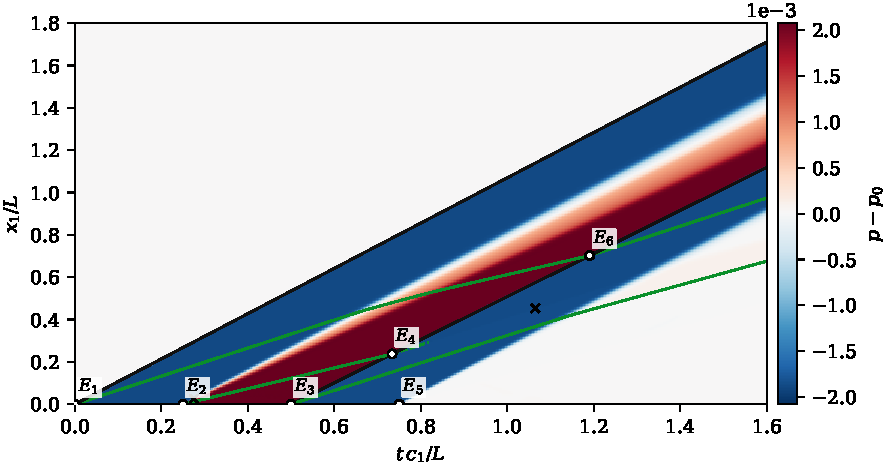
\includegraphics[width=\textwidth]{figures/xt_zoom.pdf}
\caption{Диаграмма $t$--$x$ начального участка: цвет --- $p-p_0$ (синий --- дополнительное сжатие,
красный --- растяжение); чёрные линии --- выделенные квазипродольные разрывы, зелёные ---
квазипоперечные, штрих --- узкий веер, ведомый одним разрывом; $\circ$ --- события $E_k$ (точные
задачи), $\times$ --- веер отдан сетке.}\label{fig:xt}
\vspace{4mm}
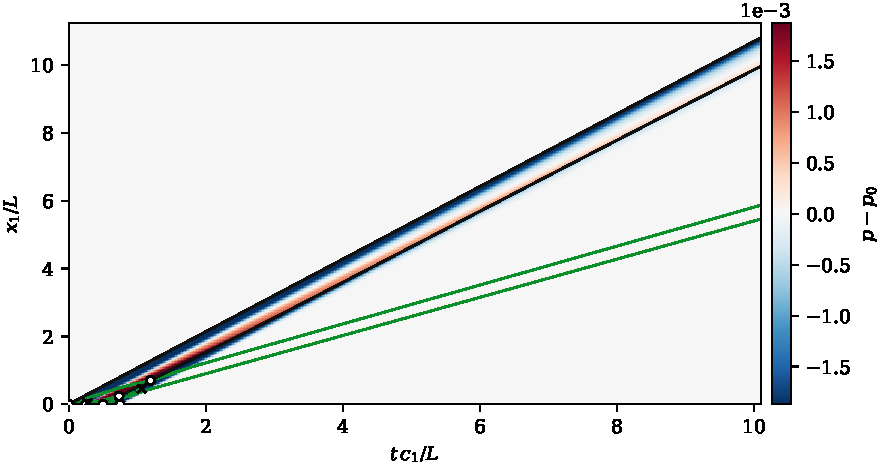
\includegraphics[width=\textwidth]{figures/xt_full.pdf}
\caption{То же на всём интервале расчёта.}\label{fig:xtfull}
\end{figure}

\begin{figure}[t]
\centering
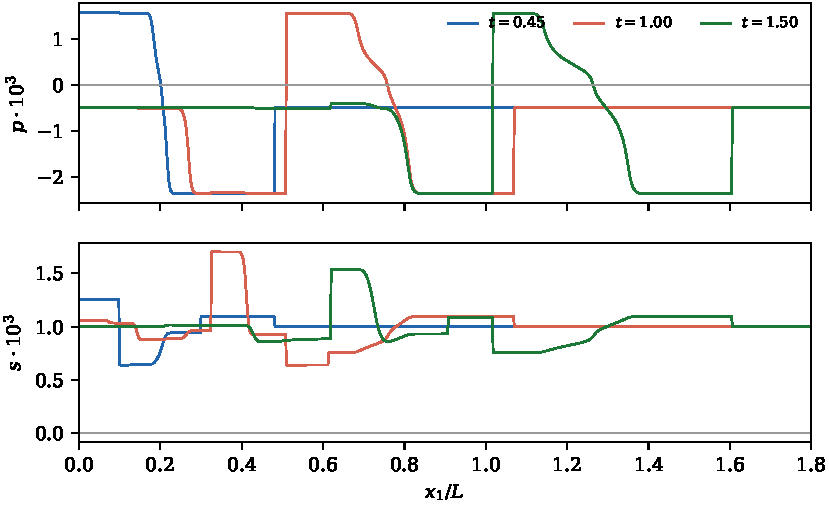
\includegraphics[width=\textwidth]{figures/profiles.pdf}
\caption{Профили $p(x)$ и $s(x)$ в моменты $t=0{,}45;\ 1{,}0;\ 1{,}5$.}\label{fig:prof}
\end{figure}

Журнал точных задач (скрипт \texttt{app/scripts/model-case.ts}) приведён в табл.~\ref{tab:events}.
Ниже --- что происходит в каждом событии и между ними.

\begin{table}[t]
\centering\footnotesize
\setlength{\tabcolsep}{3.5pt}
\caption{События разбираемого варианта: точные задачи и их исход. $G$ --- скорость (для веера ---
по крайним состояниям), $|\jump{\bF}|$ --- скачок деформации; <<сетка>> --- волна не выделяется.}\label{tab:events}
\begin{tabular}{@{}l p{1.75cm} p{3.0cm} p{2.6cm} r r p{2.3cm}@{}}
\toprule
& $t$, $x$ & что встретилось & рождённая волна & $G$ & $|\jump{\bF}|$ & ведение\\
\midrule
$E_1$ & $0$, $0$ & граница: $d\colon 0\to0{,}002$ & $f$, ударная & $1{,}0695$ & $1{,}87\cdot10^{-3}$ & выделена\\
      &          &                               & $s$, ударная & $0{,}6638$ & $1{,}53\cdot10^{-4}$ & выделена\\
$E_2$ & $0{,}25$, $0$ & граница: $d\colon 0{,}002\to-0{,}002$ & $f$, веер & $1{,}0173$ & $3{,}94\cdot10^{-3}$ & разрыв, с $t=0{,}275$ сетка\\
      &          &                               & $s$, ударная & $0{,}4907$ & $6{,}09\cdot10^{-4}$ & выделена\\
$E_3$ & $0{,}5$, $0$ & граница: $d\colon -0{,}002\to0{,}002$ & $f$, ударная & $1{,}0165$ & $3{,}95\cdot10^{-3}$ & выделена\\
      &          &                               & $s$, ударная & $0{,}6506$ & $7{,}41\cdot10^{-4}$ & выделена\\
$E_4$ & $0{,}7335$, $0{,}2374$ & $f$-ударная ($E_3$) догоняет & $f\to$, ударная & $1{,}0171$ & $3{,}93\cdot10^{-3}$ & выделена\\
      &          & $s$-ударную ($E_2$)           & $s\to$, \textbf{веер} & $0{,}6519$ & $7{,}56\cdot10^{-4}$ & разрыв, с $t=1{,}065$ сетка\\
      &          &                               & $s\leftarrow$, отражённая & $-0{,}6364$ & $2{,}4\cdot10^{-5}$ & сетка ($<1\,\%$)\\
      &          &                               & $f\leftarrow$, отражённая & $-1{,}0749$ & $1{,}5\cdot10^{-7}$ & сетка ($<1\,\%$)\\
$E_5$ & $0{,}75$, $0$ & граница: $d\colon 0{,}002\to0$ & $f$, веер & $1{,}0718$ & $1{,}86\cdot10^{-3}$ & сетка\\
      &          &                               & $s$, веер & $0{,}5696$ & $1{,}55\cdot10^{-4}$ & сетка\\
$E_6$ & $1{,}1904$, $0{,}7021$ & $f$-ударная ($E_3$) догоняет & $f\to$, ударная & $1{,}0171$ & $3{,}94\cdot10^{-3}$ & выделена\\
      &          & $s$-ударную ($E_1$)           & $s\to$, ударная & $0{,}6640$ & $1{,}65\cdot10^{-4}$ & выделена\\
      &          &                               & $s\leftarrow$, $f\leftarrow$, отражённые & & $5{,}8\cdot10^{-6}$, $3{,}9\cdot10^{-8}$ & сетка\\
\bottomrule
\end{tabular}
\end{table}

\paragraph{$E_1$, удар ($t=0$).} Граница начинает вдавливаться со скоростью $d=0{,}002$. Краевая
задача даёт две ударные волны сжатия. Быстрая ($G=1{,}0695$) переводит среду из $p_0=-0{,}0005$
в $p=-0{,}00237$. Медленная ($G=0{,}6638$) почти не меняет $p$, но меняет сдвиг: $s$ от
$0{,}00109$ к $0{,}00094$, $v_3$ гасится до нуля, как требует условие на границе. Скорость
быстрой волны лежит между $c_f(p_0)=1{,}035$ впереди и $c_f=1{,}080$ позади --- условие Лакса.

\paragraph{$E_2$, рывок ($t=0{,}25$).} Скорость границы меняется на $-0{,}002$: среда у границы
переходит из сжатия ($p=-0{,}00237$) в растяжение ($p=+0{,}00156$). Быстрая волна ---
\emph{разгрузочный веер через $p=0$}. Его характеристические скорости меняются от $c_f=1{,}080$
(фронт, в сжатой зоне) до $0{,}922$ (тыл, в растянутой): веер быстро расширяется. Пока он уже
размазывания сетки \eqref{eq:thin}, он ведётся одним разрывом, а при $t=0{,}275$ отдаётся сетке
(<<$\times$>> на рис.~\ref{fig:xt}). Медленная волна при этом --- \emph{ударная}
($G=0{,}4907$): в растянутой среде $c_s$ мало, и скачок сдвига $s$ от $0{,}00065$ к $0{,}00125$
сжимающий для этого семейства. Это проявление разномодульности: при одном и том же воздействии
быстрая волна разгружает, а медленная образует ударную волну.

\paragraph{Между $E_2$ и $E_4$: веер обгоняет ударные волны $E_1$.} Голова веера ($c_f=1{,}080$)
быстрее быстрой ударной волны $E_1$ ($1{,}0695$), но догнала бы её лишь при
$1{,}080(t-0{,}25)=1{,}0695\,t$, т.е. $t\approx25$ --- за пределами расчёта. Поэтому лидирующая волна
идёт до конца без изменений (рис.~\ref{fig:xtfull}). Медленную ударную волну $E_1$ веер обгоняет
целиком. Это непрерывное взаимодействие \eqref{eq:front}: впереди неё среда становится растянутой,
скорость падает с $0{,}664$ до $0{,}472$, амплитуда --- с $1{,}5\cdot10^{-4}$ до $1{,}25\cdot10^{-4}$.

\paragraph{$E_3$, повторный удар ($t=0{,}5$).} Из растяжения ($p=+0{,}00158$) граница снова
вдавливается. Быстрая ударная волна соединяет растянутое и сжатое состояния ($p$ от $+0{,}00158$ до
$-0{,}00234$): это <<разномодульная>> ударная волна. Её скорость $1{,}0165$ лежит между $c_f$
растянутой ($0{,}922$) и сжатой ($1{,}080$) среды. Медленная ударная волна ($G=0{,}6506$) снова
гасит $v_3$.

\paragraph{Ударная волна $E_3$ в веере $E_2$.} Быстрая ударная волна $E_3$ входит в растянутую
часть веера $E_2$ и <<съедает>> его. Впереди неё состояние постепенно возвращается к сжатому, скачок
уменьшается (с $3{,}9\cdot10^{-3}$ до $1{,}0\cdot10^{-3}$ к $t=10$), скорость растёт до $1{,}048$, затем
снова падает до $1{,}038$ (рис.~\ref{fig:xtfull}). Событий здесь нет: всё описывает
\eqref{eq:front}, а отражённые слабые волны уходят в сетку.

\paragraph{$E_4$: быстрая ударная волна догоняет медленную ($t=0{,}7335$).} Ударная волна $E_3$
догоняет медленную ударную волну рывка $E_2$. Распад разрыва даёт продолжение быстрой ударной волны
и --- главное --- \emph{смену типа медленной волны}. Позади быстрой ударной волны среда снова
сжата, и та же медленная волна (скачок $s$ от $0{,}00170$ к $0{,}00095$) в сжатой среде оказывается
\emph{разрежением}, то есть веером. Сначала он ведётся одним разрывом (штрих на рис.~\ref{fig:xt}),
при $t=1{,}065$ отдаётся сетке. Отражённые к границе волны слабы ($2{,}4\cdot10^{-5}$ и
$1{,}5\cdot10^{-7}$, меньше $1\,\%$ встретившихся) и остаются сетке.

\paragraph{$E_5$, остановка границы ($t=0{,}75$).} Скорость границы обнуляется: из сжатого
состояния уходят два разгрузочных веера (быстрый и медленный). Оба широкие и сразу считаются сеткой.
Состояние у границы возвращается почти к исходному ($p=-0{,}000485$, $s=0{,}00106$).

\paragraph{$E_6$: быстрая ударная волна догоняет медленную ударную волну $E_1$ ($t=1{,}19$).}
Медленная ударная волна первого удара, ослабленная и замедленная веером $E_2$ (она в растянутой
среде, $G=0{,}472$), встречается с быстрой ударной волной $E_3$. После встречи медленная волна
оказывается в сжатой среде и остаётся ударной, но ускоряется до $0{,}664$. Отражения пренебрежимо
малы.

\paragraph{Далее.} Выделенных встреч больше нет: лидирующая быстрая ударная волна ($1{,}0695$),
быстрая ударная волна $E_3$, ослабляемая веером, и медленные ударные волны расходятся. Режим
<<до затухания>> останавливает расчёт при $t=10{,}11$, а гладкие волны разгрузки продолжают
обгонять и ослаблять ударные волны.

\paragraph{Балансы.} Кинематический баланс выполнен до $4\cdot10^{-16}$. Работа границы
$3{,}419\cdot10^{-6}$ (в единицах $(\lambda+2\mu)L$) раскладывается так:
\begin{center}
\begin{tabular}{lr}
\toprule
прирост энергии среды & $1{,}115\cdot10^{-6}$ ($32{,}6\,\%$)\\
диссипация на выделенных ударных волнах \eqref{eq:D} & $2{,}122\cdot10^{-6}$ ($62{,}1\,\%$)\\
численная диссипация (сетка) & $0{,}182\cdot10^{-6}$ ($5{,}3\,\%$)\\
\bottomrule
\end{tabular}
\end{center}
Численная часть убывает при измельчении сетки (в похожем варианте со слабым предсжатием
$7{,}7\to4{,}4\to2{,}5\,\%$ при удвоении числа ячеек). Её источники --- размазывание вееров на сетке
(ограничитель у их краёв) и ударные волны, которые могут образоваться на сетке из волн сжатия и не
выделяются (см. ограничения).

%======================================================================
\section{Проверка формул}\label{sec:verify}

\subsection{Формальная проверка в Lean 4}
Файл \texttt{docs/model/lean/DudkoModel/Basic.lean} содержит 26 теорем о вещественных числах
(Lean~4.36, Mathlib), перечисленных в приложении~\ref{app:lean}. Сборка
\texttt{lake build} проходит без \texttt{sorry}. Команда \texttt{\#print axioms} показывает, что
каждая теорема опирается только на стандартные аксиомы (\texttt{propext}, \texttt{Classical.choice},
\texttt{Quot.sound}).

\emph{Что это гарантирует.} Каждая алгебраическая формула статьи и кода (инварианты, вектор
напряжений, условия на разрыве и формула скорости, тождество диссипации, спектр акустической матрицы,
квадратный корень, характеристический поток, граничное состояние, явные решения линеаризованных задач)
следует из явно выписанных гипотез без ошибок. \emph{Чего это не гарантирует.} Существование и
единственность решений \emph{нелинейных} задач о распаде разрыва, допустимость ударных волн при
невыпуклости, сходимость схемы --- это утверждения анализа. Их формализация --- отдельная большая
работа. Для них ниже приведены численные проверки.

\subsection{Численные проверки}
Тесты \texttt{app/tests/model.test.ts} и \texttt{app/tests/hybrid.test.ts} (запуск \texttt{npm test}):
\begin{itemize}
\item $\bT=\partial W/\partial\bF$ (конечные разности потенциала), согласие \eqref{eq:T} с полным
тензором \eqref{eq:sigma}, симметрия и положительная определённость $A$ --- для обоих материалов в
сжатых и растянутых состояниях;
\item разномодульность: $c_f>1{,}07$ при сжатии и $c_f<0{,}92$ при растяжении (материал~2);
\item ударные волны краевой задачи удовлетворяют \eqref{eq:rh} с точностью $10^{-12}$, обе формы
\eqref{eq:D} совпадают, $\mathcal D>0$; <<ударная волна разрежения>> дала бы $\mathcal D<0$;
\item $C^2=A$; граничное состояние \eqref{eq:bstate} --- предел точной краевой задачи (отличие второго
порядка по $\Delta v$);
\item амплитуды распада малого разрыва совпадают с явной формулой \eqref{eq:linrp} до $10^{-12}$;
\item удар сжатием: выделенные ударные волны совпадают с автомодельным решением §2.3 до 9 знаков;
\item широкий веер сходится к точному решению при измельчении сетки;
\item серия из трёх ударов совпадает с методом волновых фронтов (материал~1 --- до $10^{-5}$,
материал~2 --- до $3\cdot10^{-4}$ по $L_1$), балансы выполнены;
\item структура волн разбираемого варианта (табл.~\ref{tab:events}): типы волн в событиях
$E_1$--$E_5$, смена типа в $E_4$, кинематический баланс.
\end{itemize}

\subsection{Ограничения модели и метода}
\begin{itemize}
\item Ударные волны, образующиеся на сетке из волн сжатия (опрокидывание), не распознаются и не
выделяются. Сетка ведёт их со своей численной диссипацией; вместе с размазыванием вееров это даёт
$\approx5\,\%$ невязки энергии.
\item Сходимость в широких веерах --- около первого порядка (из-за точек рождения вееров и
ограничителя).
\item Модель одномерна, нейтральная волна (поворот сдвига при $g_0\neq0$) не рассматривается.
\item Потенциал \eqref{eq:W} неаналитичен при $J_2=0$. В варианте $J_2\ge s^2/2>0$ всюду, но
состояния с $s\to0$ при $p\to0$ требуют отдельного рассмотрения.
\end{itemize}

%======================================================================
\appendix
\section{Перечень формально проверенных утверждений}\label{app:lean}
\small
\begin{longtable}{@{}p{0.36\textwidth}p{0.6\textwidth}@{}}
\toprule
Теорема Lean & Утверждение\\
\midrule
\endhead
\multicolumn{2}{@{}l}{\emph{A.1. Одномерная деформация}}\\
\lean{J1_eq}, \lean{J2_eq}, \lean{J3_eq} & инварианты \eqref{eq:J} для $\varepsilon=\begin{psmallmatrix}p&g/2&s/2\\g/2&0&0\\s/2&0&0\end{psmallmatrix}$\\
\lean{traction_eq} & вектор напряжений \eqref{eq:T} из закона \eqref{eq:sigma}\\
\multicolumn{2}{@{}l}{\emph{A.2. Условия на разрыве}}\\
\lean{rh_iff} & $\jump{\mathbf f}=G\jump{\bw}\iff \jump{\bv}=-G\jump{\bF},\ \jump{\bT}=G^2\jump{\bF}$\\
\lean{shock_speed} & коллинеарность $\jump{\bT}\parallel\jump{\bF}$ и формула \eqref{eq:G2}\\
\lean{linear_shock_is_characteristic} & для $\bT=A\bF$: $\det(A-G^2I)=0$ или $\jump{\bF}=0$\\
\multicolumn{2}{@{}l}{\emph{A.3. Энергия}}\\
\lean{dissipation_identity} & $\jump{\bT\cdot\bv}+G\jump{E} = G(\jump{W}-\avg{\bT}\cdot\jump{\bF})$ при \eqref{eq:rh}\\
\lean{energy_balance_moving_jump} & изменение энергии на отрезке с движущимся разрывом $=$ приток $-\ \mathcal D\,\Delta t$\\
\lean{weak_shock_cubic} & $\jump{W}-\avg{T}\jump{F}=-k_3\jump{F}^3/12$ для кубического $W$\\
\multicolumn{2}{@{}l}{\emph{A.4. Спектр акустической матрицы}}\\
\lean{eigen_char} & $\lambda_\pm$ \eqref{eq:eig} --- корни $\det(A-\lambda I)$\\
\lean{eigen_vec} & $(b,\lambda-a)$ --- собственный вектор\\
\lean{eigen_orth} & $\br_+\perp\br_-$\\
\lean{eigen_pos} & $A>0\Rightarrow 0<\lambda_-\le\lambda_+$ (гиперболичность)\\
\multicolumn{2}{@{}l}{\emph{A.5. Квадратный корень}}\\
\lean{sqrt_sq}, \lean{sqrt_det} & для \eqref{eq:sqrt}: $C^2=A$, $\det C=\sqrt{\det A}$\\
\lean{sqrt_comm} & $CA=AC$\\
\multicolumn{2}{@{}l}{\emph{A.6. Поток}}\\
\lean{simple_wave_dir} & $J(\br,-\sigma\br)=\sigma(\br,-\sigma\br)$ при $A\br=\sigma^2\br$\\
\lean{jacobian_sq} & $J^2=\operatorname{diag}(A,A)$\\
\lean{flux_consistent} & $\mathbf f^*(\bw,\bw)=\mathbf f(\bw)$\\
\lean{ghost_flux} & поток через границу с фиктивной ячейкой равен $-\bv^*$\\
\multicolumn{2}{@{}l}{\emph{A.7. Граница}}\\
\lean{riemann_invariant} & $\mathbf q=\bv+C\bF$: $\mathbf q_t - C\mathbf q_x=0$ для линейной акустики с $A=C^2$\\
\lean{boundary_state} & $\bv_b+C\bF_b=\bv+C\bF\Rightarrow \bF_b=\bF-C^{-1}(\bv_b-\bv)$\\
\multicolumn{2}{@{}l}{\emph{A.8. Линеаризованные задачи}}\\
\lean{lin_riemann_solution} & явное решение \eqref{eq:linrp}\\
\lean{lin_riemann_unique} & однородная задача имеет только нулевое решение\\
\lean{lin_boundary_solution} & явное решение \eqref{eq:linbp}\\
\bottomrule
\end{longtable}
\normalsize

\section{Воспроизведение}
\begin{itemize}
\item Тесты: \texttt{cd app \&\& npm test}.
\item Журнал и данные рисунков: \texttt{cd app \&\& node} \nolinkurl{scripts/model-case.ts} \nolinkurl{../docs/model/figures/case.json},
затем \texttt{python3 docs/model/figures/make\_figures.py}.
\item Lean: \texttt{cd docs/model/lean \&\& lake build} (Lean~4.36.0-rc2, Mathlib \texttt{v4.36.0-rc2}).
\item Статья: \texttt{cd docs/model \&\& latexmk -pdf model.tex}.
\end{itemize}

\end{document}
